\documentclass[12pt, tikz]{beamer}

\usetheme[progressbar=frametitle]{metropolis}
\usepackage{appendixnumberbeamer}
\usepackage{graphicx,wrapfig}
\usepackage[export]{adjustbox}
\usepackage{pgfplots}
\usepackage{verbatim}
\usepackage{graphicx}
\usepackage[backend=bibtex, style=authoryear]{biblatex}
\bibliography{thesis}
\usepackage{tikz}
\usepackage{listings}
\usepackage{xcolor}
\usepackage{caption}
\usepackage[normalem]{ulem}
\usepackage{dirtree}
\usetikzlibrary{graphdrawing}
\usetikzlibrary{graphs}
\usepackage{subcaption}

\setbeamercolor{block title}{bg=gray!50}
\setbeamercolor{block body}{bg=gray!30}
\setbeamercolor{block title example}{fg={rgb:green,1;black,2}}
\setbeamercolor{block body example}{fg={rgb:green,1;black,2}}

\setbeamercolor{background canvas}{bg=white}

\definecolor{darkblue}{rgb}{0.0,0.0,0.6}
\definecolor{bracket}{RGB}{130,130,130}
\definecolor{quote}{RGB}{150,50,50}

\lstset{
  basicstyle=\ttfamily\scriptsize,
  columns=fullflexible,
  showstringspaces=false,
  commentstyle=\color{gray}\upshape
}

\usepackage[most]{tcolorbox}

\setbeamertemplate{footline}[text line]{
	\parbox{\linewidth}{\vspace*{-8pt} \hfill\insertpagenumber}}
\setbeamertemplate{navigation symbols}{}

\title{Comparing Conditional Random Fields and LSTM Networks for Named Entity Recognition}	
\date{\today}

\author{Josef Gugglberger (student),
\and Sara Bauer (supervisor),
\and Clemens Sauerwein (supervisor)}
\institute{LV 703605-6 Masterseminar
\and 
\includegraphics[scale=0.3]{img/universitaet-innsbruck-logo-rgb-farbe}}

\begin{document}
	
% titel
\begin{frame}
\maketitle
\end{frame}

\begin{frame}[fragile]{Motivation}
	\begin{center}
	James visited the Eiffel Tower in 2012.\\
	\pause
	$\downarrow$ \\
	\pause
	\textcolor{red}{James} \scalebox{0.4}{[PERSON]} visited the \textcolor{green}{Eiffel} \scalebox{0.4}{[LOCATION]} \textcolor{green}{Tower} \scalebox{0.4}{[LOCATION]} in \textcolor{blue}{2012} \scalebox{0.4}{[TIME]}.	
	\end{center}
	\pause
	\begin{itemize}
		\item traditional approach was machine learning (CRF, HMM, etc.)
		\item from 2015 onwards deep learning is considered state of the art for many NLP tasks
	\end{itemize}
\end{frame}

\begin{frame}[fragile]{Goal of Thesis}
	
	\begin{block}{Goal of Thesis}
		Apply a practical study comparing Conditional Random Fields and Long-Short-Term-Memory Networks for Named Entity Recognition. The aim is to implement both approaches and compare their precision, recall and F1-score on two different datasets. 
	\end{block}
\end{frame}

% überblick
\begin{frame}{Overview}
\setbeamertemplate{section in toc}[sections numbered]
\tableofcontents[hideallsubsections]
\end{frame}


\section{Background}

\begin{frame}[fragile]{Named Entity Recognition}
	\begin{block}{Definition: NER}
		\textit{Named Entity Recognition} is the task of locating and classifying named entities in unstructured text. A named entity is classified into a predefined set of categories.
	\end{block}
	\pause
	\begin{center}
		James visited the Eiffel Tower in 2012.\\
		$\downarrow$ \\
		\textcolor{red}{James} \scalebox{0.4}{[PERSON]} visited the \textcolor{green}{Eiffel} \scalebox{0.4}{[LOCATION]} \textcolor{green}{Tower} \scalebox{0.4}{[LOCATION]} in \textcolor{blue}{2012} \scalebox{0.4}{[TIME]}.	
	\end{center}
\end{frame}

\begin{frame}[fragile]{Conditional Random Fields}
	\begin{block}{Definition: CRF \footcite{lafferty2001conditional}}
	A \textit{Conditional Random Field} is a discriminative probabilistic classifier. It makes its prediction not just based on the input sample, but also based on the context of the input sample.
	\end{block}
	\pause
	\vspace{-0.35cm}
	\begin{equation}
	p(y|x) = \frac{1}{Z(x)} \prod_{t=1}^T exp(\sum_{k=1}^{K} \theta_k f_k(y_t, y_{t-1}, x_t))
	\end{equation}

	where $Z(x)$ is an normalization function:

	\begin{equation}
	Z(x) = \sum_{y} \prod_{t=1}^{T} exp(\sum_{k=1}^{K} \theta_k f_k(y_t, y_{t-1}, x_t))
	\end{equation}
\end{frame}

\begin{frame}[fragile]{Recurrent Neural Networks}
	
	\begin{block}{Definition: RNN}
		RNNs are a special type of artificial neural networks that have a feedback loop feeding the hidden layers back into themselves. The loop provides a kind of memory that allow the network to better recognize patterns.
	\end{block}
	\pause
	\vspace{0.5cm}
	\begin{overprint}
		\onslide<2> 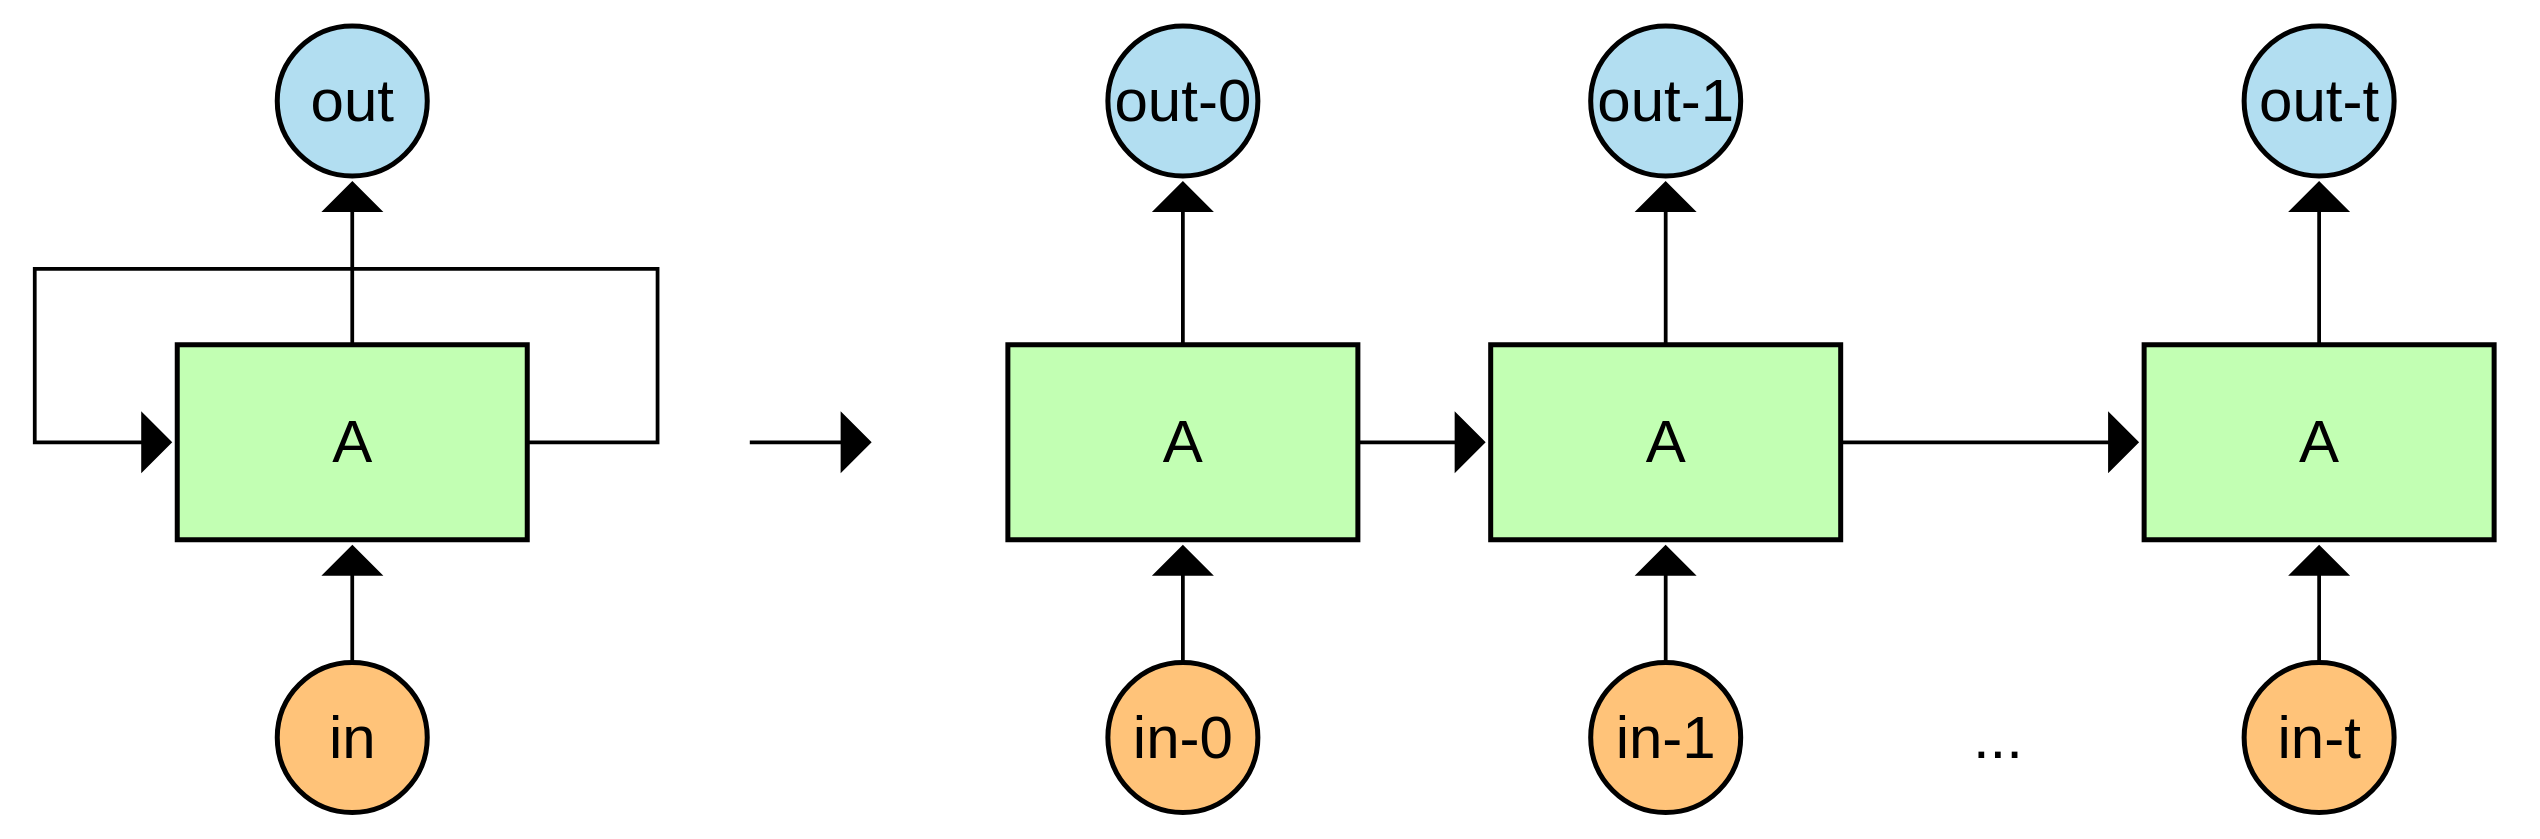
\includegraphics[width=\linewidth]{img/rnn.png}
		\onslide<3->
		\begin{itemize}
			\item<3-> Suited for sequence labeling
			\item<4-> Problems with long term dependencies
			\begin{itemize}
				\item Vanishing and exploding gradient
			\end{itemize}
		\end{itemize}
	\end{overprint}

\end{frame}

\begin{frame}[fragile]{Long-Short-Term-Memory Networks}

	\begin{block}{Definition: LSTM\footcite{hochreiter1997long} networks}
		LSTM networks are a special type of RNNs, which where designed to overcome issues with the vanishing gradient on long term relationships.
	\end{block}
	\pause
	\vspace{-0.5cm}
	\begin{center}
		\begin{figure}
			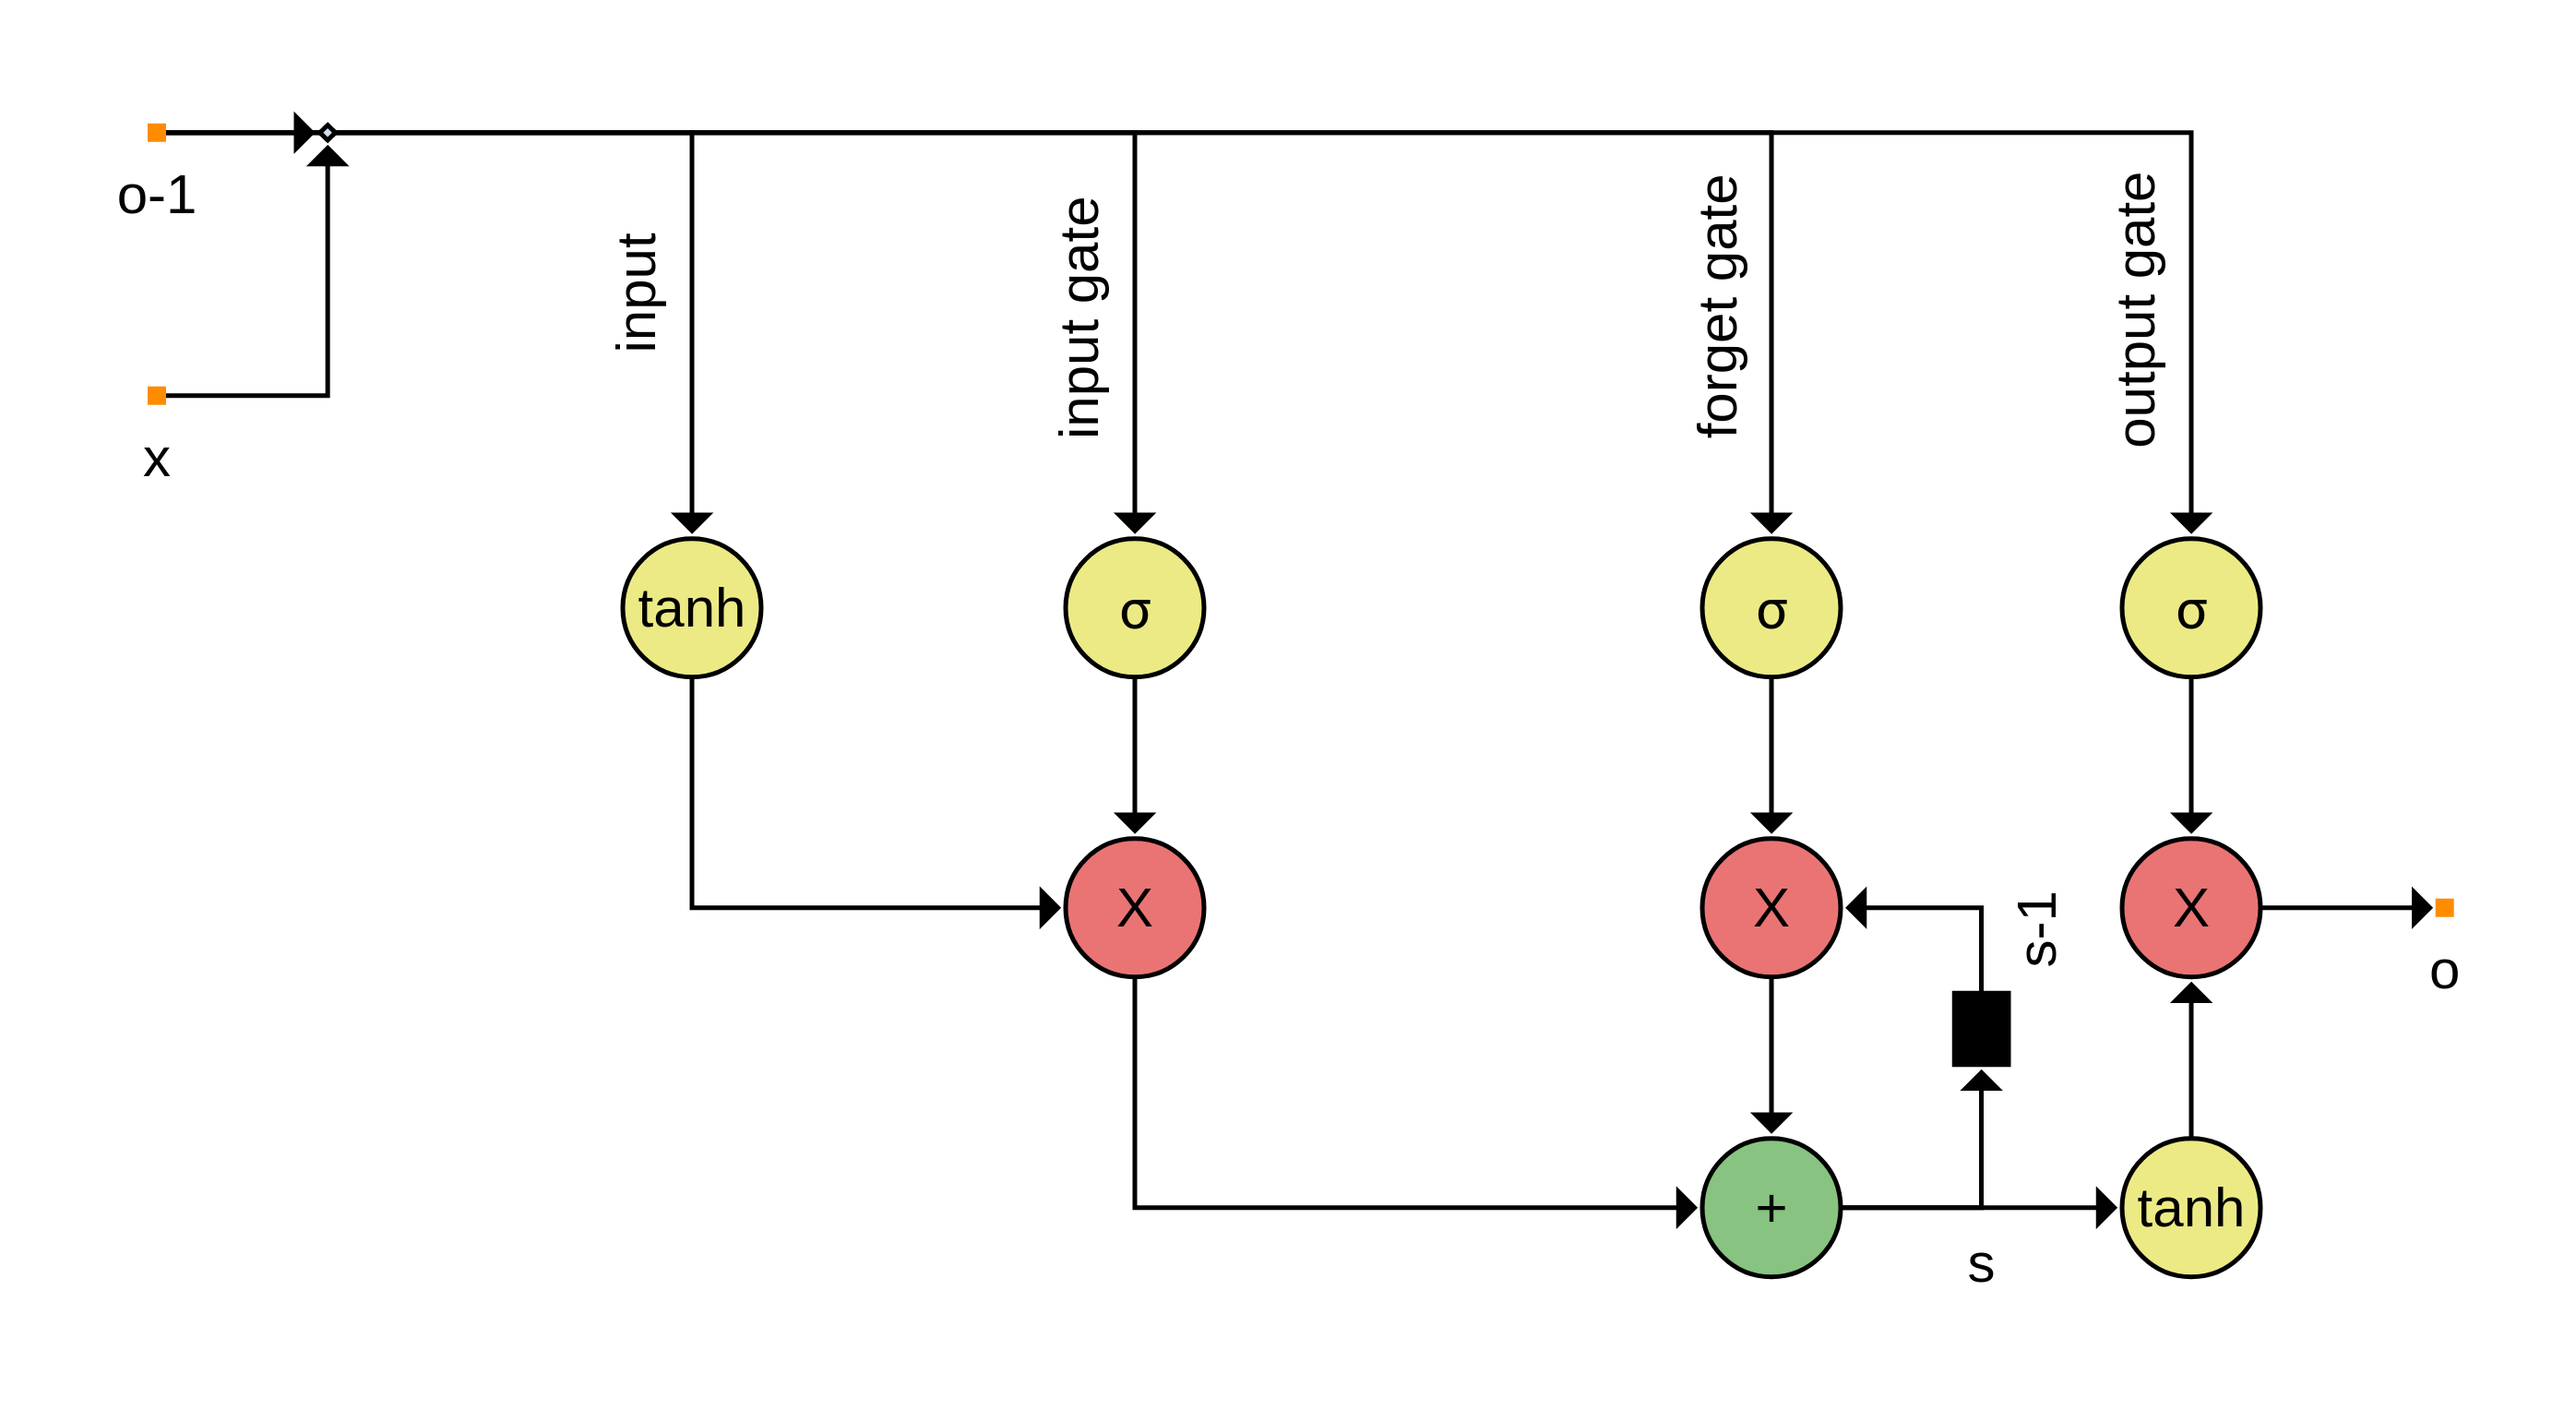
\includegraphics[width=0.9\linewidth]{img/lstm.png}
		\end{figure}
	\end{center}
\end{frame}

\section{Implementation Details}

\begin{frame}[fragile]{Dataset CoNLL}
	
	\begin{block}{Conference on Computational NL Learning}
		CoNLL 2003 \footcite{tjongkimsang2003conll} was a shared task on language independent named entity recognition. The data is based on news wire articles from the Reuters corpus.
	\end{block}
	\pause
	Four types of Named Entities:
	\begin{itemize}
		\item Person
		\item Location
		\item Organization
		\item Miscellaneous
	\end{itemize}

\end{frame}

\begin{frame}[fragile]{Dataset W-NUT}
	
	\begin{block}{Workshop on Noisy User-generated Text}
		W-NUT 17 \footcite{derczynski2017results} was a workshop that focused on NLP on noisy and informal text, such as comments from social media, online reviews, forums, etc.
	\end{block}
	\pause
	Six types of Named Entities:
	\begin{itemize}
		\item Person
		\item Location
		\item Corporation
		\item Consumer good
		\item Creative work
		\item Group 
	\end{itemize}
	
\end{frame}

\begin{frame}[fragile]{Dataset Syntax}
	\begin{center}
		\begin{table}
		\begin{tabular}{l | l | l | l}
			Word & POS* & Syntax Chunk* & NE \\
			\hline
			U.N. & NNP & I-NP & I-ORG 
\\
			official & NN & I-NP & O 
\\
			Ekeus & NNP & I-NP & I-PER \\ 
			heads & VBZ & I-VP & O 
\\
			for & IN & I-PP & O \\
			Baghdad & NNP & I-NP & I-LOC \\ 
			. & . & O & O \\
		\end{tabular}
		\caption{Starred columns are optional.}
		\end{table}
	\end{center}
\end{frame}

\begin{frame}[fragile]{Conditional Random Fields}
	Libraries:
	\begin{itemize}
		\item pycrfsuite
		\item nltk
		\item gensim
	\end{itemize}
	\pause
	
	Features should describe characteristics of named entities:
	\begin{itemize}
		\item<2-> Word Features
		\item<3-> Sentence \& Collection Features
		\item<4-> Dictionary Features
		\item<5-> Features from unsupervised ML algorithms
	\end{itemize}
\end{frame}

\begin{frame}[fragile]{Word Features}
	\begin{itemize}
		\item<1-> length of word
		\item<2-> the word starts with an upper-case letter
		\item<3-> the word contains an upper-case letter
		\item<4-> the word contains a digit
		\item<5-> the word contains a special character (-, /, etc.)
		\item<6-> word shape: 'Word' $\rightarrow$ 'Aa+', 'WORD' $\rightarrow$ 'A+', '2019-12-12' $\rightarrow$ '9999\#99\#99'
	\end{itemize}
\end{frame}

\begin{frame}[fragile]{Sentence \& Collection Features}
	\begin{itemize}
		\item<1-> position of word in sentence
		\item<2-> number of occurrences in collection
	\end{itemize}
\end{frame}

\begin{frame}[fragile]{Dictionary Features}
	The word is contained in:
	\begin{itemize}
		\item<1-> \textbf{stop-words} list
		\begin{itemize}
			\item is, as, the, are, has, that, etc.
			\item Problems: 'The Who', 'Take That'
		\end{itemize}
		\item<2-> \textbf{name list}
		\begin{itemize}
			\item 7579 person names form nltk corpus
		\end{itemize}
		\item<3-> \textbf{word list}
		\begin{itemize}
			\item dictionary of 235892 words from nltk corpus
		\end{itemize}
		\item<4-> \textbf{WordNet}
		\begin{itemize}
			\item dictionary and thesaurus
			\item provides hypernyms, synonyms, etc.
		\end{itemize}
	\end{itemize}
\end{frame}

\begin{frame}[fragile]{Features from unsupervised ML algorithms}
	
	The cluster of each word is used as a feature.
	
	\alt<1>{
	\begin{itemize}
		\item \textbf{brown cluster}
		\begin{itemize}
			\item hierarchical clustering algorithm
		\end{itemize}
	\end{itemize}
	
	\centering
	\includegraphics[width=0.5\linewidth]{img/brown.png}
	}{
	\begin{itemize}
		\item brown cluster
	\end{itemize}
	}
	\alt<2>{
	\begin{itemize}
		\item \textbf{Latent Dirichlet Allocation} (LDA) \footcite{blei2003latent} topic
		\begin{itemize}
			\item modelling the abstract topics of document
			\item example: document A is 20\% topic 1, 60\% topic 2 and 20\% topic 3
		\end{itemize}
	\end{itemize}
	}{
	\begin{itemize}
		\item Latent Dirichlet Allocation (LDA)
	\end{itemize}
	}
	\alt<3>{
	\begin{itemize}
		\item \textbf{gensim implementation of w2v cluster}
		\begin{itemize}
			\item maps similar words to similar vectors
			\item $w2v(king) - w2v(man) + w2v(woman) = \sim w2v(queen)$
		\end{itemize}
	\end{itemize}
	}{
	\begin{itemize}
		\item w2v cluster
	\end{itemize}
	
	}
\end{frame}

\begin{frame}[fragile]{LSTM Network}
	Libraries:
	\begin{itemize}
		\item Keras functional API
		\item Tensorflow as backend
	\end{itemize}
	\pause
	\vspace{-0.3cm}
	\begin{figure}
		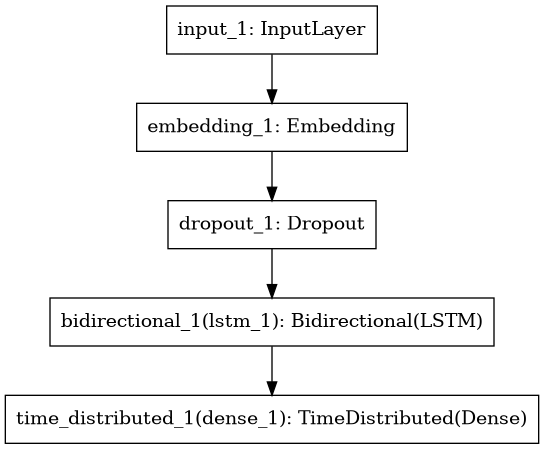
\includegraphics[width=0.6\textheight]{img/lstm_model.png}
		\caption{LSTM model, as presented in \footcite{huang2015bidirectional}}
	\end{figure}
\end{frame}

\begin{frame}[fragile]{Bidirectional LSTM Layer}
	\begin{itemize}
		\item<1-> idea is to duplicate LSTM layer
		\begin{itemize}
			\item<2-> input as-is is feed into first LSTM layer
			\item<3-> input reversed is feed into second LSTM layer
		\end{itemize}
		\item<4-> speech depends on context of past and future
	\end{itemize}

	\onslide<5->
	\begin{exampleblock}{Example}
		The other day we saw Paris \uncover<5>{.} \uncover<6->{\hspace{-0.25cm}\textcolor{red}{Hilton.}}
	\end{exampleblock} 
\end{frame}

\begin{frame}[fragile]{Time Distributed Dense Layer}
	\begin{itemize}
		\item adds the same dense layer to every timestep 
	\end{itemize}
	\pause
	\begin{figure}
		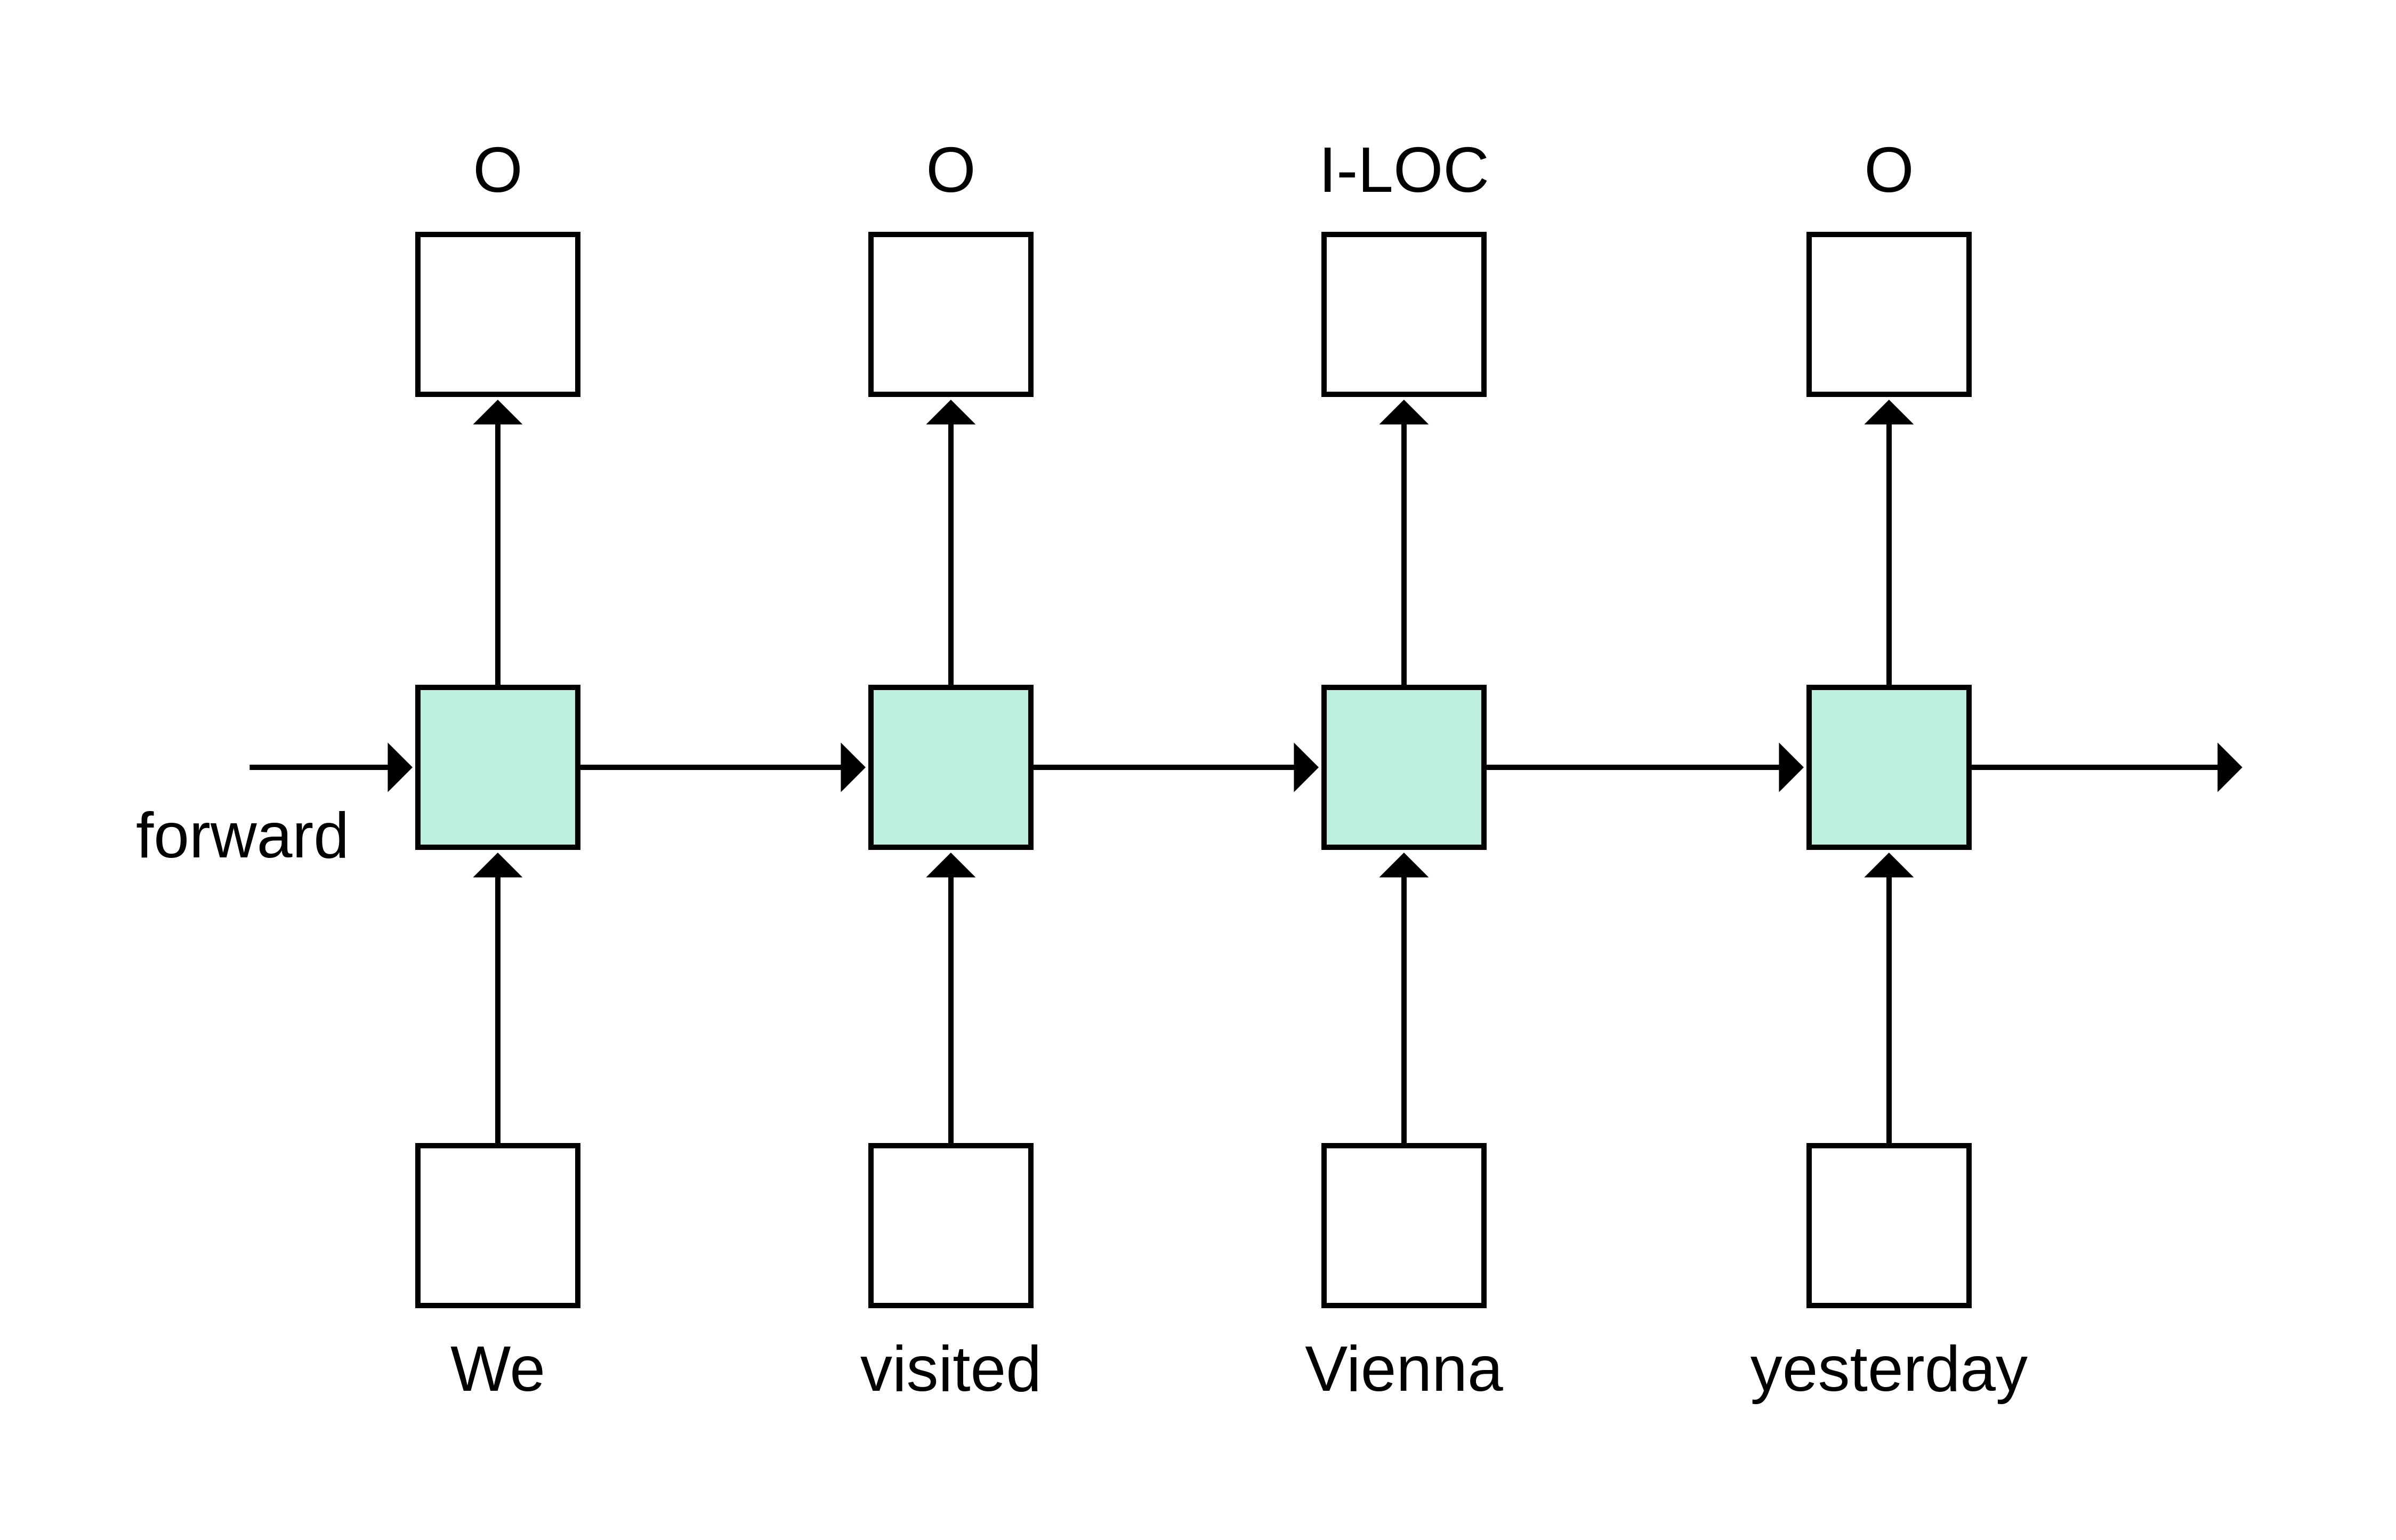
\includegraphics[width=\linewidth]{img/lstm_overview.png}
	\end{figure}
\end{frame}

\begin{frame}[fragile]{The best of both worlds?}
	combine LSTM network with CRF  \footcite{huang2015bidirectional}:
	\begin{itemize}
		\item<1-> use past input features via LSTM layer
		\item<2-> use sentence level tag information via CRF layer
	\end{itemize}

	\vspace{-0.2cm}
	\onslide<3->
	\centering
	\begin{figure}
		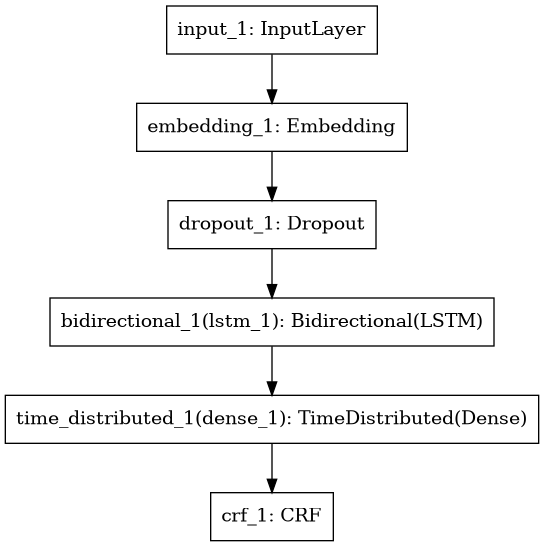
\includegraphics[width=0.5\linewidth]{img/lstm_crf_model.png}
	\end{figure}
\end{frame}


\section{Evaluation and Comparison}

\begin{frame}[fragile]{Evaluation}
	Evaluation of the implemented NER systems with metrics:
	\begin{itemize}
		\item precision
		\item recall
		\item F1-score
	\end{itemize}

	\pause
	
	Evaluation performed based on named entity level.
\end{frame}

\begin{frame}[fragile]{Results}
	CoNLL dataset:
	\begin{center}
		\begin{tabular}{| l | c | c | c |}
			\hline
			Method & Precision & Recall & F1-score \\ \hline
			CRF & 84.25 & 85.42 & 84.83 \\ \hline
			Bi-LSTM* & 84.37 & \textbf{86.58} & 85.46 \\ \hline
			Bi-LSTM-CRF* & \textbf{89.41} & 86.20 & \textbf{87.78} \\ \hline
		\end{tabular}
	\end{center}

	W-NUT dataset:
	\begin{center}
	\begin{tabular}{| l | c | c | c |}
		\hline
		Method & Precision & Recall & F1-score \\ \hline
		CRF & 31.54 & \textbf{56.72} & \textbf{40.53} \\ \hline
		Bi-LSTM & 8.69 & 23.16 & 12.63 \\ \hline
		Bi-LSTM-CRF* & \textbf{33.61} & 31.03 & 32.27 \\ \hline
	\end{tabular}
\end{center}

{\footnotesize * pre-trained GloVe-embeddings used}

\end{frame}

\begin{frame}[fragile]{State-of-the-art in NER}
	\begin{figure}
		
\includegraphics[width=0.2\linewidth]{img/flair.png}
	\end{figure}
	\begin{itemize}
		\item<1-> State-of-the-art NLP tool (by Zalando Research \footcite{akbik2019flair})
		\item<2-> uses Bi-LSTM-CRF model
		\item<3-> 93.09 F1 on CoNLL 2003
		\item<4-> 49.49 F1 on W-NUT 2017
	\end{itemize}
\end{frame}


\section{Conclusion}

\begin{frame}[fragile]{Conclusion}
	\begin{itemize}
		\item<1-> CRF approach needs a lot of feature engineering
		\item<2-> training CRF is not really faster because of unsupervised clustering algorithms
		\item<3-> for noisy text CRFs seems to work better
		\item<4-> LSTM approach has more potential for improvement
		\begin{itemize}
			\item use additional input layers
			\item use other string embeddings (Flair, BERT, ELMo)
		\end{itemize}
	\end{itemize}
\end{frame}


%\printbibliography

\end{document}